\chapter{Resultaten}
De resultaten van het project zijn ...\\

Een resultaten van enkele testvluchten zijn te vinden op figuur \ref{fig:test_flight_1}, \ref{fig:test_flight_2}, \ref{fig:test_flight_3}, \ref{fig:test_flight_4}.\\
\begin{figure}[p]
	\centering
	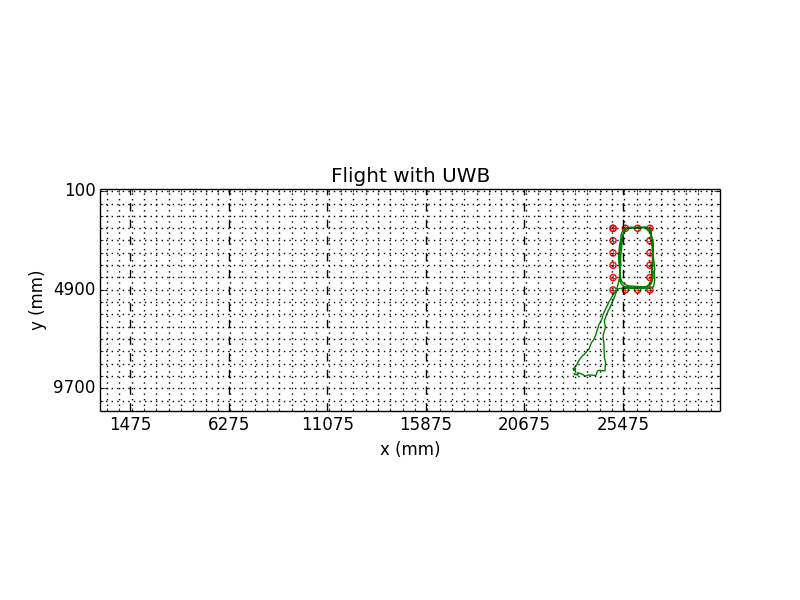
\includegraphics[width=\textwidth]{Test_Flight_1}
	\caption[Testvlucht 1]{Testvlucht 1.}
	\label{fig:test_flight_1}
	
	\centering
	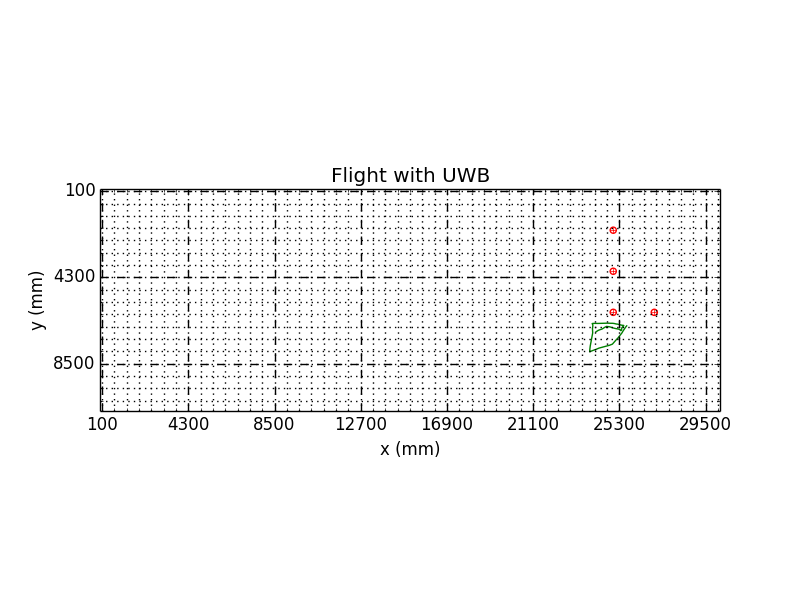
\includegraphics[width=\textwidth]{Test_Flight_2}
	\caption[Testvlucht 2]{Testvlucht 2.}
	\label{fig:test_flight_2}
\end{figure}
\begin{figure}[p]
	\centering
	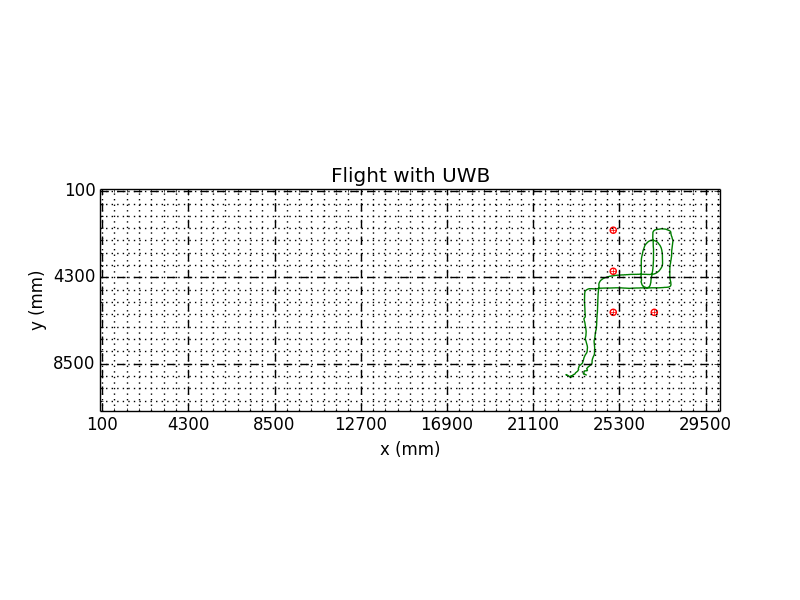
\includegraphics[width=\textwidth]{Test_Flight_3}
	\caption[Testvlucht 3]{Testvlucht 3.}
	\label{fig:test_flight_3}

	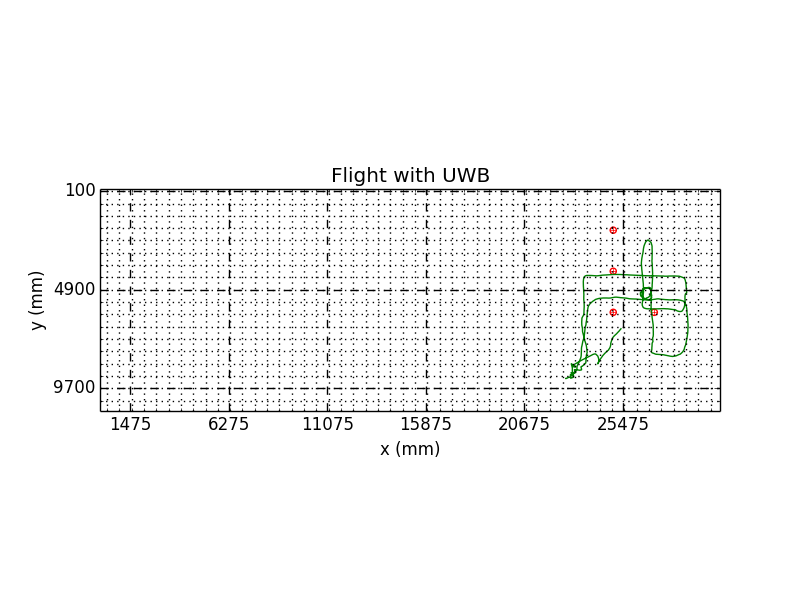
\includegraphics[width=\textwidth]{Test_Flight_4}
	\caption[Testvlucht 4]{Testvlucht 4.}
	\label{fig:test_flight_4}
\end{figure}

Een openstaand probleem van het project is dat het verbinden van de off-board controller met 2 verschillende netwerken nog niet optimaal verloopt. Vaak wil de ene applicatie niet verbinden met het juiste netwerk.

Een tekort aan het project is dat de drone momenteel altijd moet opstarten met de voorkant wijzend naar de positieve x-as. Dit kan manueel niet altijd even nauwkeurig gebeuren waardoor vaker correcties moeten gebeuren tijdens een vlucht. Dit is van toepassing op beide algoritmes.\\
Een mogelijke oplossing voor dit probleem is om de drone op een bepaald punt in de ruimte vast te zetten zodat de lengte van de drone parallel ligt met de x-as, met de voorkant richting het positieve deel.\\
Een andere oplossing is om de drone eerst te calibreren alvorens de vlucht aan te vatten.
Hierbij kun je eerst een aantal meter recht vooruit vliegen en vervolgens checken in welke richting de drone gevlogen heeft.
Dit brengt enkele veronderstellingen met zich mee, die haast onmogelijk in werkelijkheid gereproduceerd kunnen worden. bijvoorbeeld: de drone moet recht vooruit vliegen, zonder af te wijken door luchtstromingen of te roteren tijdens de vlucht.
Ook heb je een relatief grote plaats nodig waar je in alle mogelijke richtingen enkele meters kan vliegen.\\


\section{Kosten}
Hier komt de verantwoording van gemaakte kosten.\\
De extra batterij van \SI{1000}{\mA\hour} was nodig om op korte tijd voldoende te kunnen testen. Zonder die extra batterij zou er telkens meer dan een uur gewacht moeten worden na een kwartier testen.\\
De eerste LiPo batterijen (van \SI{150}{\mA\hour}) die aangekocht werden bleken niet lang genoeg stroom te kunnen leveren aan de on-board controller. Daarna kozen we voor veel grotere batterijen van \SI{500}{\mA\hour}.\\
De aankoop van de Adafruit HUZZAH bleek overbodig nadat de controller opgesplitst werd. Ook zou het niet meer mogelijk geweest zijn om de gekozen libraries te gebruiken.\\

Een overzicht van alle gemaakte kosten vindt u in tabel \ref{tab:kosten}.\\
Niet alles staat hier in verwerkt. Zo werden de Pozyx location anchors en tags vrij verkregen, alsook de Raspberry Pis.
\begin{table}[p]
\centering
\begin{tabular}{ |l|r|r|r| } \hline
Product & Prijs (\euro{}) & Aantal & Totaal (\euro{}) \\ [.5ex] \hline \hline
Parrot AR.Drone 2.0 Elite Edition & 116.71 & 1 & 116.71 \\ \hline
Micro USB OTG & 1.32 & 2 & 2.64 \\ \hline
5 LiPo batterijen \SI{150}{\mA\hour} en lader voor controller & 12.47 & 1 & 12.47 \\ \hline
Adafruit HUZZAH & 14.57 & 1 & 14.57 \\ \hline
LiPo batterij \SI{1000}{\mA\hour} voor drone & 34.99 & 1 & 34.99 \\ \hline
2 LiPo batterijen \SI{500}{\mA\hour} en lader voor controller & 35.35 & 1 & 35.35 \\ [.5ex] \hline
Velcro & 0.79 & 1 & 0.79 \\ \hline
\hline
Totaal & & & 218.16 \\ \hline
\end{tabular}
\caption[Kosten]{Verantwoording van gemaakte kosten.}
\label{tab:kosten}
\end{table}